\documentclass[11pt,a4paper]{article}
\usepackage[finnish]{babel}
\usepackage[utf8]{inputenc}
\usepackage{graphicx}


\author{Marko Haanranta}
\date{\today}
\title{Tietorakennevertailun testiraportti}

\begin{document}
\maketitle
Projektissa toteutin binäärikeon, binomikeon, fibonaccin keon ja AVL-puun. Lisäksi käytin vertailussa apunani priority queue:ta. 
Testaamisen toteutin yksikkö- ja suorituskykytestein.
\section{Yksikkötestaus}
Jotta tietorakenteita oli mahdollista vertailla keskenään niin ensin oli varmistuttava, että toteuttamani tietorakenteet toimivat oikein. Tätä varten tein kattavat yksikkötestit kaikille toteuttamilleni tietorakenteille. Lause- ja haaraumakattavuuden varmistamiseen käytin cobertura työkalua.

Binomikeko, fibonaccin keko ja AVL-puun solmuilla on useita eri parametreja joten ne oli järkevää toteuttaa olioina. Näille solmu luokille ei tehty omia yksikkötestejä, koska niissä ei ole muita metodeja kun gettereitä ja settereitä joiden testaamista ei katsota tarpeelliseksi. Coberturaa käyttäen voi kuitenkin havaita, että näidenkin luokkien testikattavuus on lähes 100\%
\section{Suorituskykytestaus}
Tätä varten testasin delete ja insert metodien nopeuksia suurilla syötteillä. Pienimmän alkion haku, kun ei poisteta mitään on kaikilla rakenteilla sen verran nopea operaatio etten katsonut sen testaamisen olevan tarpeellista.
\subsection{Tilavaativuudet}
Tilavaativuus kaikkien toteutettujen tietorakenteiden osalta on O(1), koska mikään toiminnallisuutta toteuttava metodi ei käytä kuin vakiotilaisia apumuuttujia.
\subsection{Aikavaativuudet}
Teoreettiset aikavaativuudet poikkeavat hieman toisistaan. Kaikkien toteutettujen tietorakenteiden poisto operaation teoreettinen aikavaativuus on O(logn). Fibonaccin keon lisäys operaation teoreettinen aikavaativuus on O(1)(amortized). 

Javan valmiin priority queue-tietorakenteen lisäys ja poisto operaatioille luvataan O(logn) aikavaativuus, joten näin voin kätevästi vertailla toimivatko toteuttamini tietorakenteet niin nopeasti kuin niiden teoreettisesti tulisi toimia.
\subsection{Testisyötteet ja testien toteutus}
Testeissä syötin tietorakenteisiin tietyn määrän 100-30 000 000 avainta ja mittasin miten kauan lisäys ja poisto operaatiot veivät aikaa.
\section{Testitulokset}
Yleisesti ottaen kaikki toteuttamani tietorakenteet toimivat riittävän hyvin paitsi lisäys fibonaccin kekooon, josta lisää myöhemmin.
\subsection{Avainten lisäys}
Kaikki toteuttamani tietorakenteet olivat nopeampia kuin javan priority queue, joten niiden voi sanoa toimivan O(logn) ajassa. Fibonaccin keon lisäys operaatiolle luvataan kuitenkin O(1)(amortized) aikavaativuus. Suorittamieni testien mukaan tämä ei toteutunut vaan fibonaccin kekoon lisääminen oli samaa luokkaa muiden tietorakenteiden kanssa. Nopeiten alkioita voi lisätä binomikekoon.
\begin{figure}[h]
\centering
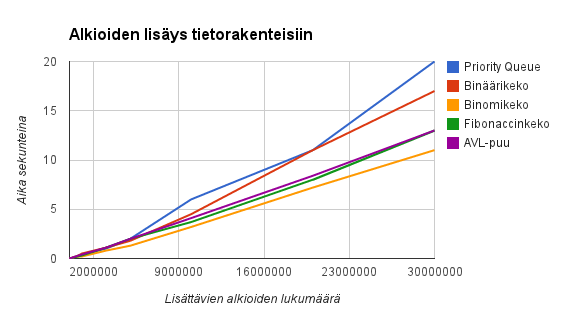
\includegraphics[scale=0.7]{alkioidenlisays.png}
\caption{Alkioiden lisäys tietorakenteisiin}
\end{figure}
\subsection{Avainten poisto}
Avainten poisto tietorakenteista sai selkeästi enemmän eroja aikaan kuin lisäys. Poisto operaatio vei kuitenkin hitaimmastakin rakenteesta tehty 30 000 000 avaimen poisto vei kuitenkin vain 3 kertaa enemmän kuin priority queue:sta poisto, joten toteuttamieni tietorakenteiden poisto operaation voi sanoa toimivan O(logn) ajassa. Binäärikeosta poistaminen oli selkeästi hitain operaatio. Nopeinta poistaminen oli AVL-puusta ja binomikeko pärjäsi myös hyvin.
\begin{figure}[h]
\centering
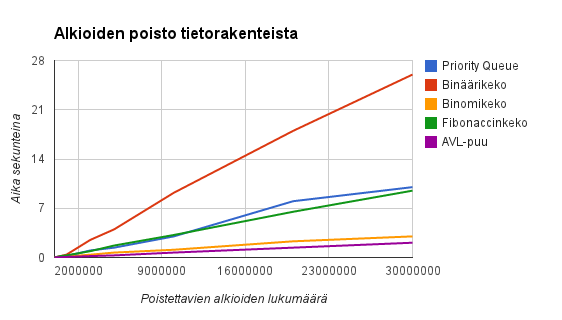
\includegraphics[scale=0.7]{alkioidenpoisto.png}
\caption{Alkioiden poisto tietorakenteista}
\end{figure}
\section{Jyvät ja akanat}
Tekemäni testaamisen perusteella parhaat tietorakenteet olivat binomikeko ja AVL-puu. Sekä alkioiden lisäämien, että poistaminen hoitui suuhteellisen nopeasti verrattuna muihin tietorakenteisiin. Jos pelkästään halutaan olla varmoja nopeasta lisäämisestä niin sitten joko binomikeko tai fibonaccin keko ovat hyvät valinnat. Jos taas ainoastaan halutaan olla varmoja, että avaimet voi poistaa nopeasti niin sitten AVL-puu on paras valinta. 
\section{Kritiikkiä}
Testaaminen antoi kuvan, että fibonaccin kekoon lisääminen ei toimi niin nopeasti kuin sen teoreettisesti pitäisi. Tähän voisi vaikuttaa testitapa. Tein testit lisäämällä valtavan määrän avaimia kerralla ja vasta kun kaikki on lisätty niin aletaan poistaminen. Fibonaccin keko rakentuu keoksi vasta poistojen yhteydessä, joten ennen kuin alkioita poistetaan se on vain pitkä kahteen suuntaan linkitetty juurisolmulista.
Pienillä syötteillä fibonaccin kekoon lisääminen oli hieman nopeampaa kuin muihin toteuttamiini tietorakenteisiin.
\end{document}